\documentclass{report}
\usepackage[utf8]{inputenc}
\usepackage{lmodern} % Fonte Latin Modern
\usepackage[T1]{fontenc} % Codificação da Saída
\usepackage[brazil]{babel}
\usepackage{subfig}
\usepackage{graphicx}
\usepackage{amsfonts}
\usepackage{amssymb}
\usepackage{amsmath}
\usepackage{multicol}
\usepackage{ifthen}
\newboolean{firstanswerofthechapter}  
\usepackage{xcolor}
\colorlet{lightcyan}{cyan!40!white}
\usepackage{chngcntr}
\usepackage{stackengine}
\usepackage{tasks}
\usepackage{multirow}
\usepackage{booktabs}
\usepackage{float}
\newlength{\longestlabel}
\settowidth{\longestlabel}{\bfseries viii.}
%\settasks{counter-format={tsk[r].}, label-format={\bfseries}, label-width=\longestlabel,
    %item-indent=0pt, label-offset=2pt, column-sep={10pt}}
		
% \setcounter{secnumdepth}{0} \setlength{\topmargin}{0cm}
% \setlength{\headsep}{-2cm} \setlength{\textwidth}{17.5cm}
% \setlength{\textheight}{23cm} \setlength{\oddsidemargin}{-0.8cm}
% \setlength{\evensidemargin}{0cm} \setlength{\footskip}{-1.5cm}

\usepackage[left=1.5cm,right=1.5cm,top=2cm,bottom=0.5cm,includefoot]{geometry}
		
\usepackage[lastexercise,answerdelayed]{exercise}
%\counterwithin{Exercise}{chapter}
%\counterwithin{Answer}{chapter}
%\renewcounter{Exercise}[chapter]
%\newcommand{\QuestionNB}{\bfseries\arabic{Question}.\ }
%\renewcommand{\ExerciseName}{Exercício}
%\renewcommand{\ExerciseHeader}{\noindent\def\stackalignment{l}% code from https://tex.stackexchange.com/a/195118/101651
    %\stackunder[0pt]{\colorbox{cyan}{\textcolor{white}{\textbf{\LARGE\ExerciseHeaderNB\;\large\ExerciseName}}}}{\textcolor{lightcyan}{\rule{\linewidth}{2pt}}}\medskip}
\renewcommand{\ExerciseName}{Exercícios}
\renewcommand{\ExerciseHeader}{\noindent\def\stackalignment{l}% code from https://tex.stackexchange.com/a/195118/101651
    \stackunder[0pt]{\colorbox{gray}{\textcolor{white}{\textbf{\large\ExerciseName}}}}{\textcolor{lightgray}{\rule{\linewidth}{2pt}}}\medskip}
%\renewcommand{\AnswerName}{Exercises}
%\renewcommand{\AnswerHeader}{\ifthenelse{\boolean{firstanswerofthechapter}}%
    %{\bigskip\noindent\textcolor{cyan}{\textbf{CHAPTER \thechapter}}\newline\newline%
        %\noindent\bfseries\emph{\textcolor{cyan}{\AnswerName\ \ExerciseHeaderNB, page %
                %\pageref{\AnswerRef}}}\smallskip}
    %{\noindent\bfseries\emph{\textcolor{cyan}{\AnswerName\ \ExerciseHeaderNB, page \pageref{\AnswerRef}}}\smallskip}}
%\setlength{\QuestionIndent}{16pt}

\usepackage{Sweave}
\begin{document}
\input{Lista1-concordance}


\vspace*{-2cm}

\begin{center}
\begin{minipage}[s]{4cm}
\hspace{-1.3cm}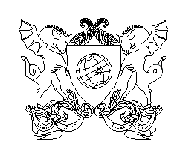
\includegraphics[scale=1.0]{Figuras/brasaoufv.eps}
\end{minipage}
\begin{minipage}[s]{13cm}
{\begin{center} {\sc \Large Universidade Federal de Vi\c{c}osa}\\
{\sc \large Instituto de Ci\^encias Exatas e Tecnológicas}\\
{\sc \large Campus UFV - Florestal}\\
\end{center}}
\end{minipage}\begin{minipage}[s]{2 cm}
%\includegraphics[width=2 cm]{logoimecc.eps}
\end{minipage}
\end{center}

\vspace{-0.3cm}

%\hline \hline \noindent

%%%%%%%%%%%%%%%%%%%%%%%%%%%%%%%%%%%%%%%%%%%%%%%%%%%%%%%%%%%%%%%%%%%%%%%%%%%

\medskip

\begin{center}

\underline{\underline{{\large{\sc Lista de Iniciação Estatística - Lista 1}}}}

\bigskip

{\large {\bf Prof. Fernando Bastos}}
%\bigskip
%
\end{center}

\begin{Exercise}

\Question Represente as somas utilizando somatórios:
\begin{tasks}(2)
\task $x_{1}y_{1}+x_{2}y_{2}+\cdots x_{10}y_{10};$
\task $1+2+3+4+5+\cdots$
\task $1+2^{3}+3^{4}+4^{5}+\cdots+100^{101};$
\task $1+2^{2}+3^{3}+\cdots+30^{30};$
\task $\dfrac{1}{z_{1}}+\dfrac{2}{z_{2}}+\cdots+\dfrac{r}{z_{r}};$
\task $\dfrac{1}{2}+\dfrac{2}{3}+\cdots+\dfrac{n}{n+1};$
\task $(a_{2}-b_{1})+(a_{3}-b_{2})+\cdots+(a_{50}-b_{49});$
\task $a_{0}+a_{1}x+a_{2}x^{2}+\cdots+a_{10x^{10}};$
\end{tasks} 
$\newline$
\Question Desenvolva cada uma das somas indicadas:
\begin{tasks}(2)
\task ${\displaystyle \sum_{j=1}^{6}x_{j}};$
\task ${\displaystyle \sum_{i=1}^{6}(x_{i}-k)};$
\task ${\displaystyle \sum_{i=2}^{10}k};$
\task ${\displaystyle \sum_{j=1}^{10}z_{j}(z_{j}+2)};$
\task ${\displaystyle \sum_{i=1}^{4}x_{i}^{2}};$
\task ${\displaystyle \sum_{i=1}^{5}x_{i}^{2-i}};$
\task ${\displaystyle \sum_{j=1}^{6}5j};$
\task ${\displaystyle \sum_{i=-2}^{2}i^{3}};$
\end{tasks} 
$\newline$
\Question Verdadeiro ou Falso:
\begin{tasks}(2)
\task (\ ) ${\displaystyle \sum_{i=0}^{200}i^{3}=\sum_{i=1}^{200}i^{3}};$
\task (\ ) ${\displaystyle \sum_{i=0}^{n}i=\dfrac{n(n+1)}{2}};$
\task (\ ) ${\displaystyle \sum_{i=0}^{n}i^{2}=\dfrac{n(n+1)(2n+1)}{6}};$
\task (\ ) ${\displaystyle \sum_{s=0}^{1000}(3+s)=3+\sum_{s=0}^{1000}s};$
\task (\ ) ${\displaystyle \sum_{k=1}^{n}2k=2\sum_{k=1}^{n}k};$
\task (\ ) ${\displaystyle \sum_{i=0}^{n}i^{2}=\Biggl(\sum_{i=0}^{n}i\Biggl)^{2}};$
\task (\ ) ${\displaystyle \sum_{l=8}^{32}(3+l)=75+\sum_{l=8}^{32}l};$
\task (\ ) ${\displaystyle \sum_{i=5}^{200}(a_{i}+b_{i})=\sum_{i=5}^{m}a_{i}+\sum_{i=5}^{m}b_{i}};$
\end{tasks}

\newpage

\Question Sabendo-se que ${\displaystyle \sum_{i=1}^{10}X_{i}=-6}$ e que 
${\displaystyle \sum_{i=1}^{10}X_{i}^{2}=12},$ calcule:

\begin{tasks}(2)
\task  ${\displaystyle \dfrac{\displaystyle\sum_{i=1}^{10}X_{i}^{2}-\dfrac{\left(\displaystyle\sum_{i=1}^{10}X_{i}\right)^{2}}{10}}{10-1}}$
\task  ${\displaystyle \sum_{i=1}^{10}X_{i}(X_{i}-2)}$
\task  ${\displaystyle \sum_{i=1}^{10}(X_{i}-3)^{2}}$
\task  ${\displaystyle \sum_{i=1}^{10}(4X_{i}+5)}$
\task  ${\displaystyle \sum_{i=1}^{10}(X_{i}-4)}$
\task  ${\displaystyle \sum_{i=1}^{10}(X_{i}-4)^{2}}$
\task  ${\displaystyle \dfrac{ \sum_{i=1}^{10}(X_{i}-4)^{2}}{10-1}}$
\task  ${\displaystyle \dfrac{\sum_{i=1}^{10}X_{i}}{10}}$
\end{tasks}
$\newline$
\Question Utilizando os dados da tabela abaixo, referente aos valores $X_{ij}$ calcule o resultado numérico quando possível:

$$
\begin{tabular}{c|cccc}
  \hline
  % after \\: \hline or \cline{col1-col2} \cline{col3-col4} ...
  i$\setminus$ j & 1 & 2 & 3 & 4 \\
  \hline
  1 & 8 & 7 & 5 & 9 \\
  2 & 4 & 0 & 10 & 2 \\
  \hline
\end{tabular}
$$

\begin{tasks}(2)
\task  ${\displaystyle \sum_{i=1}^{2}X_{i1}}$
\task  ${\displaystyle \sum_{j=1}^{4}X_{1j}}$
\task  ${\displaystyle \sum_{j=1 \atop j\neq 3}^{4}X_{ij}}$
\task  ${\displaystyle \sum_{j=2}^{3}X_{2j}}$
\task  ${\displaystyle \sum_{j=1 \atop j\neq 2}^{4}\dfrac{1}{X_{2j}}}$
\task  ${\displaystyle \prod_{j=1 \atop j\neq 3}^{4}6X_{1j}}$
\task  ${\displaystyle \prod_{j=1 \atop j\neq 2}^{4}X_{2j}}$
\end{tasks}
$\newline$
\Question Escrever usando notação de somatório ou produtório, conforme o caso:

\begin{tasks}(2)
\task ${\displaystyle \left(\dfrac{X_{1}-Y_{1}}{2}+\dfrac{X_{2}-Y_{2}}{2}+\dfrac{X_{4}-Y_{4}}{2}\right)^{2}}$
\task ${\displaystyle a!}$
\task ${\displaystyle (X_{1}+Y_{1})(X_{1}+Y_{2})(X_{1}+Y_{3})}$
\task ${\displaystyle (X_{1}Y_{1})+(X_{1}Y_{2})+(X_{1}Y_{3})+(X_{2}Y_{1})+(X_{2}Y_{2})+(X_{2}Y_{3})}$
\task ${\displaystyle (X_{1}Y_{1}).(X_{2}Y_{2}).\ldots.(X_{n}Y_{n})}$
\task ${\displaystyle x_{1}^{2}+x_{2}^{2} \cdots x_{n}^{2}}$
\task ${\displaystyle [(b_{1}-2):(w_{1}+4)]^{8}+\cdots+[(b_{20}-2):(w_{20}+4)]^{8}}$
\task ${\displaystyle a_{1}b_{1}+a_{3}b_{3}+\cdots+a_{25}b_{25}}$
\task ${\displaystyle \log{x_{1}}+\log{x_{2}}+\cdots+\log{x_{n}}}$
\task ${\displaystyle (kx_{1})(kx_{2})(kx_{3})\cdots(kx_{n})}$
\end{tasks}
$\newline$
\Question Se $X_{1}=2,\quad X_{2}=4,\quad X_{3}=6$\quad e\quad $Y_{1}=3,\quad Y_{2}=5,\quad Y_{3}=6,$ calcule:


\begin{tasks}(2)
\task ${\displaystyle \sum_{i=1}^{3}\left(X_{i}Y_{i}\right)}$
\task ${\displaystyle \sum_{i=1}^{3}\left(X_{i}-2\right)\left(Y_{i}-5\right)}$
\end{tasks}

\newpage

\Question Identifique cada uma das variáveis seguintes como quantitativa, qualitativa
e como contínua, discreta, nominal, ordinal.

\begin{tasks}
\task O número de vitórias do corinthians no ano de 2017.
 \task A concentração de impurezas em um copo de água, em mg, por litro.
 \task A quantidade de manchas em uma camisa.
 \task O tempo de reação a um estímulo qualquer.
 \task A resposta de um indivíduo a questão: ``Qual a sua origem?''
 \task Sua idade?
 \task A vazão de uma torneira em litros por segundo.
 \task A resposta a uma pergunta com as opções de resposta:
 \begin{enumerate}
 \item[i)] Concordo plenamente;
\item[ii)] Concordo;
\item[iii)] Discordo;
\item[iv)] Discordo totalmente;
\end{enumerate}
\task o número de moradores de uma cidade.
\task A sua temperatura em um momento de febre.
\task a nota de sua primeira prova de Estatística.
\task Sua formação.
\task o número de derrotas do Atlético Mineiro nos últimos 50 anos.
\end{tasks}
$\newline$
\Question Observou-se, em um estudo sobre a quantidade de cartões amarelos recebidos por jogadores de dois times em um campeonato regional com 25 jogos os números abaixo:
\begin{table}[H]
 \begin{minipage}{.5\textwidth}
 \centering
 \caption{Torresmo FC}
 \begin{tabular}{|c|c|c|c|c|}
 \hline
  1&2&4&4&7\\ \hline
  3&3&2&4&5\\ \hline
  2&4&3&5&3\\ \hline
  2&4&3&6&5\\ \hline
  5&6&4&6&5\\ \hline
 \end{tabular}
  
 \end{minipage} 
 \begin{minipage}{.5\textwidth}
 \centering
 \caption{Tá-lento FC}
 \begin{tabular}{|c|c|c|c|c|}
 \hline
  1&7&7&6&1\\ \hline
  2&6&1&7&2\\ \hline
  1&3&2&7&5\\ \hline
  6&1&7&4&1\\ \hline
  5&7&6&3&2\\ \hline
 \end{tabular}
 \end{minipage}% 
\end{table}

\begin{tasks}
\task Construa uma distribuição de frequências para as 50 observações.
\task Construa uma distribuição de frequências para cada time.
\task Represente graficamente cada uma das distribuições.
\task Comente os resultados.
\end{tasks}
$\newline$
\Question A tabela abaixo apresenta a nota de 100 alunos em uma disciplina online.

\begin{table}[H]
\centering
\begin{tabular}{cccccccccc}
\hline
41	&	52	&	57	&	60	&	67	&	71	&	74	&	78	&	84	&	92	\\
42	&	52	&	57	&	61	&	68	&	71	&	75	&	78	&	84	&	92	\\
48	&	53	&	58	&	61	&	68	&	71	&	75	&	80	&	87	&	93	\\
48	&	54	&	58	&	63	&	68	&	71	&	76	&	80	&	88	&	93	\\
49	&	54	&	59	&	64	&	68	&	72	&	76	&	81	&	89	&	94	\\
49	&	54	&	59	&	64	&	69	&	72	&	76	&	81	&	89	&	95	\\
49	&	55	&	59	&	65	&	69	&	73	&	77	&	81	&	89	&	96	\\
51	&	56	&	59	&	66	&	70	&	73	&	77	&	82	&	89	&	97	\\
51	&	56	&	60	&	67	&	70	&	73	&	77	&	82	&	91	&	99	\\
51	&	56	&	60	&	67	&	70	&	74	&	77	&	83	&	91	&	100	\\
\hline
\end{tabular}
\end{table}
\begin{tasks}
\task Construa uma tabela de distribuição de frequências.
\task Faça uma distribuição gráfica para a distribuição de frequências.
\task Calcule a média, a mediana e o desvio-padrão.
\task Apresente um histograma dos dados, um diagrama de ramos e folhas, um esquema de cinco números e um boxplot.
\task Comente os resultados.
\end{tasks}
$\newline$
\Question Os pesos em kg de um conjunto de 25 pessoas, já ordenados do menor para o maior, são:
\begin{table}[H]
\centering
\begin{tabular}{ccccc}
\hline
10,37	&	24,82	&	32,50	&	77,85	&	85,24	\\
15,20	&	29,95	&	33,88	&	79,20	&	86,16	\\
20,87	&	31,09	&	40,00	&	80,15	&	90,87	\\
21,89	&	31,44	&	70,20	&	80,45	&	91,47	\\
23,52	&	32,43	&	76,50	&	81,54	&	93,38	\\
\hline
\end{tabular}
\end{table}

\begin{tasks}
\task Calcule a mediana e questione a sua representatividade neste contexto;
\task Verifique a instabilidade da mediana neste caso supondo a entrada ao grupo de mais uma pessoa nas duas situações seguintes:
\begin{enumerate}
\item[i)]  A pessoa pesa 20 kg;
\item[ii)] A pessoa pesa 80 kg;
\end{enumerate}
\end{tasks}
$\newline$
\Question

\begin{tasks}
\task Esboce um histograma onde média, mediana e moda coincidam;
\task Esboce um histograma onde média e mediana coincidam, mas não a moda;
\task Esboce os histogramas de duas variáveis $X$ e $Y$ com as mesmas médias mas com variâncias diferentes;
\end{tasks}
$\newline$
\Question Dispomos de uma relação de 200 aluguéis de imóveis urbanos e uma relação de 100
aluguéis rurais. Conforme distribuição abaixo:
\begin{table}[H]
\centering
\begin{tabular}{c|c|c}
\hline
Classe de aluguéis (codificados)& Zona Urbana & Zona rural\\
\hline
$2|-3$  &10&30\\
$3|-5$  &40&50\\
$5|-7$  &80&15\\
$7|-10$ &50&05\\
$10|-15$&20& 0\\
\hline
Total&200&100\\
\hline
\end{tabular}
\end{table}

\begin{tasks}
\task Construa os histogramas das duas distribuições.
\task Com base nos histogramas, discuta e compare as duas distribuições.
\end{tasks}

\newpage

\Question A MB Indústria e Comércio, desejando melhorar o nível de seus funcionários em cargos de chefia, montou um curso experimental e indicou 25 funcionários para a primeiraturma. Os dados referentes à seção a que pertencem, notas e graus obtidos no curso estão na tabela a seguir. Como havia dúvidas quanto à adoção de um único critério de
avaliação, cada instrutor adotou seu próprio sistema de aferição. Usando dados daquela tabela, responda às 
questões:

\begin{tasks}
\task Após observar atentamente cada variável, e com o intuito de resumi-las, como você
identificaria (qualitativa ordinal ou nominal e quantitativa discreta ou contínua) cada
uma das 9 variáveis listadas?
\task Compare e indique as diferenças existentes entre as distribuições das variáveis Direito,
Política e Estatística.
\task Construa o histograma para as notas da variável Redação.
\task Construa a distribuição de freqüências da variável Metodologia e faça um gráfico
para indicar essa distribuição.
\task Sorteado ao acaso um dos 25 funcionários, qual a probabilidade de que ele tenha
obtido grau A em Metodologia?
\task Se, em vez de um, sorteássemos dois, a probabilidade de que ambos tivessem tido A
em Metodologia é maior ou menor do que a resposta dada em (e)?
\task Como é o aproveitamento dos funcionários na disciplina Estatística, segundo a seção
a que eles pertencem?
\end{tasks}

\begin{table}[H]
\centering
\resizebox{0.9\textwidth}{!}{%
\begin{tabular}{c|c|c|c|c|c|c|c|c|c}
Funcionário&Seção &Administração  &Direito &Redação &Estatística  &Inglês &Metodologia &Política  &Economia\\
\hline
1  &P &8.0  &9.0 &8.6 &9.0  &B &A &9.0  &8.5\\
2  &P &8.0  &9.0 &7.0 &9.0  &B &C &6.5  &8 0\\
3  &P &8.0  &9.0 &8.0 &8.0  &D &B &9.0  &8.5\\
4  &P &6.0  &9.0 &8.6 &8.0  &D &C &6.0  &8.5\\
5  &P &8.0  &9.0 &8.0 &9.0  &A &A &6.5  &9.0\\
6  &P &8.0  &9.0 &8.5 &10.0 &B &A &6.5  &9.5\\
7  &P &8.0  &9.0 &8.2 &8.0  &D &C &9.0  &7.0\\
8  &T &10.0 &9.0 &7.5 &8.0  &B &C &6.0  &8.5\\
9  &T &8.0  &9.0 &9.4 &9.0  &B &B &10.0 &8.0\\
10 &T &10.0 &9.0 &7.9 &8.0  &B &C &9.0  &7.5\\
11 &T &8.0  &9.0 &8.6 &10.0 &C &B &10.0 &8.5\\
12 &T &8.0  &9.0 &8.3 &7.0  &D &B &6.5  &8.0\\
13 &T &6.0  &9.0 &7.0 &7.0  &B &C &6.0  &8.5\\
14 &T &10.0 &9.0 &8.6 &9.0  &A &B &10.0 &7.5\\
15 &V &8.0  &9.0 &8.6 &9.0  &C &B &10.0 &7.0\\
16 &V &8.0  &9.0 &9.5 &7.0  &A &A &9.0  &7.5\\
17 &V &8.0  &9.0 &6.3 &8.0  &D &C &10.0 &7.5\\
18 &V &6.0  &9.0 &7.6 &9.0  &C &C &6.0  &8.5\\
19 &V &6.0  &9.0 &6.8 &4.0  &D &C &6.0  &9.5\\
20 &V &6.0  &9.0 &7.5 &7.0  &C &B &6.0  &8.5\\
21 &V &8.0  &9.0 &7.7 &7.0  &D &B &6.5  &8.0\\
22 &V &6.0  &9.0 &8.7 &8.0  &C &A &6.0  &9.0\\
23 &V &8.0  &9.0 &7.3 &10.0 &C &C &9.0  &7.0\\
24 &V &8.0  &9.0 &8.5 &9.0  &A &A &6.5  &9.0\\
25 &V &8.0  &9.0 &7.0 &9.0  &B &A &9.0  &8.5\\
\hline
\multicolumn{10}{c}{(P = departamento pessoal, T = seção técnica e V = seção de vendas)}
\end{tabular}
}
\end{table}
\end{Exercise}

\end{document}
